\section{Unified Virtual Addressing}
\label{sec-uva}

In this section, we talk about the Unified Virtual Addressing (UVA) feature that we use to provide the same virtual memory for both GPU and CPU data, in order to have larger partitions of a graph per GPU. We first talk about the concept of UVA, and then we talk about how we implemented UVA in Gluon and finally we talk about the limitations and future directions with respect to this optimization. 

\subsection{UVA concept}
\begin{figure}
\centering
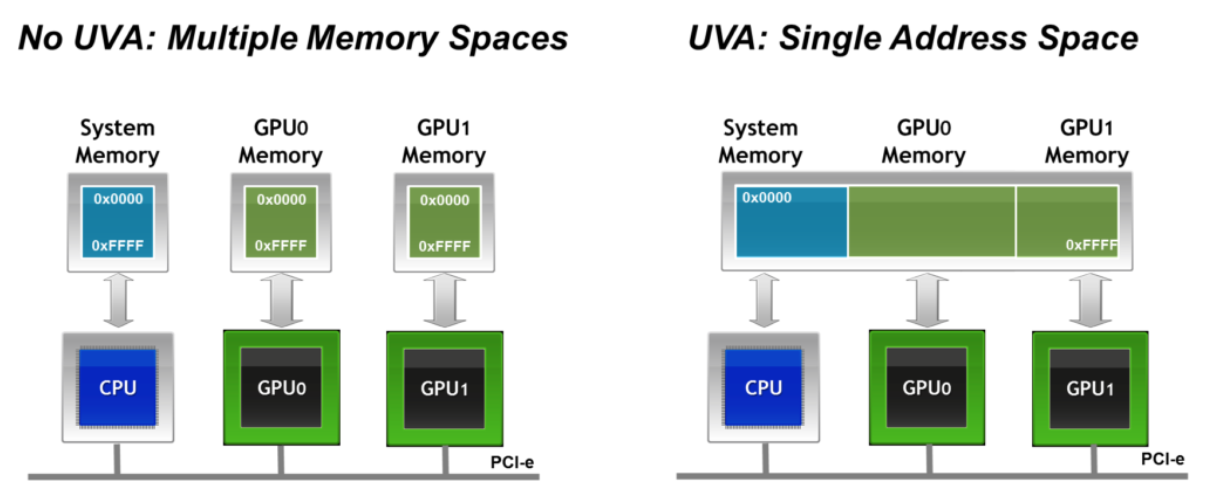
\includegraphics[width=0.49\textwidth]{uva-fig.png}
\mycaption{Unified Virtual Address}{The figure shows the address spaces with and without using UVA. 
}
\label{fig-uva}
%\vspace{-20pt}
\end{figure}

The GPU memory on servers is typically very limited. So storing graphs in GPUs places a limitation on the size of the graph per node, and requires larger clusters, increasing communication overhead and thus loss in performance. Furthermore, if we store the graphs on the host memory, then we need to copy the graphs from host memory to GPU memory and back during processing, as the address spaces of GPU memory and host memory are different. This leads to complicated implementations, and also cause overheads due to copying of data frequently between the host memory and GPU memory. To avoid this cost of copying and to store large graph partitions per GPU, NVIDIA introduced Unified Virtual Addresses (UVA). In UVA, both the GPU and the CPU memory lie in the same address space. The programmer does not need to worry about creating separate buffers for host memory and GPU memory. This is shown in Figure~\ref{fig-uva}. 

In UVA, memory is allocated in a region on the host using a call called cudaHostAlloc(). This memory is pinned memory, and cannot be paged out by the virtual memory system. Once the memory is allocated, it can be accessed from CPU as well as GPU. Note that the access of this pinned memory from GPU can be done without any copying of data from host to GPU. GPU threads can directly access and process data located in the pinned memory on the host. This technique allows you to leverage host memory when your device has limited global memory and also allows you to explicitly transfer data between host and device. 

However, sharing zero-copy memory data between host and device involves synchronizing memory accesses across host and device, because modifying data in zero-copy memory simultaneously from host and device could lead to undefined behavior. 

\subsection{Using UVA in Gluon}
We explore the use of UVA in the Gluon substrate in this project. In the original implementation of Gluon, the graph data as well as bitset and offset data is all present in the device memory. So we can imagine that for large graphs, this would lead to a problem, since the device (GPU) memory is very limited. We used Unified Virtual Addressing in which we allocated a the graph, and bitset and offset data on the host memory using cudaHostAlloc(). We then managed to use this pinned data that was allocated in the host directly for performing GPU computations, with a unified virtual address. We tested our implementation on a server with 2 GPUs, each containing 8GB of device memory. The host itself had 190GB memory. So we could potentially store 10x larger partitions on the host, as opposed to storing the graphs and the bitset and offset data entirely in the GPU. 

\subsection{Discussion and Limitations}
We stored the entire graph and all the bitset and offset data on the host memory using cudaHostAlloc(). Note that this leads to a non-trivial performance drop, since each node has to be fetched from the host through the PCI interface, instead of accessing from the fast bandwidth device memory. There is a lot of opportunity to explore smarter strategies to place only some parts of the graph which might be cold regions that are not accessed frequently using UVA, and store the hot regions in device memory. This would help us get the best of both worlds: get the high performance of device memory and also get the extra capacity from the host memory. 

Newer GPUs also support a mode called Unified Memory, which is different from Unified Virtual Addresses. The GPUs that we tested on did not have support for Unified Memory. In Unified Memory, the programmers get a similar interface as that of UVA with a single virtual address space for host and device memory. However, unified memory leads to better performance by transferring data from the host to the device when the device needs it, and managing the synchronization with the host copy of the data transparently without any efforts by the programmer. This has potential to improve the performance significantly by using smart prefetching and readahead strategies to improve the locality of data, and also gain the high capacity of host memory. 